\documentclass[12pt, xcolor={svgnames,table}]{beamer}
%\documentclass[20pt,handout]{beamer}
\usetheme{Darmstadt}
\usepackage{graphicx}
%\usepackage[german]{babel}
\usepackage{ngerman}
\usepackage[T1]{fontenc}
\usepackage[utf8]{inputenc}
\usepackage{tikz}
\setbeamertemplate{footline}[frame number]

\newcommand{\cc}[1]{\includegraphics[height=4mm]{img/#1.png}\hspace{1mm}}
\usepackage{ifthen}
\newcommand{\license}[2][]{\\#2\ifthenelse{\equal{#1}{}}{}{\\\scriptsize\url{#1}}}
\usepackage{textcomp}
\usepackage{hyperref}
%\usepackage[table]{xcolor}

\pgfdeclareimage[height=.6cm]{c3d2logo}{./img/c3d2.pdf}

\pgfdeclarelayer{foreground}
\pgfsetlayers{main,foreground}
\logo{\pgfputat{\pgfxy(-1,0)}{\pgfbox[center,base]{\pgfuseimage{c3d2logo}}}}

\title{Digitale Selbstverteidigung für Engagierte in der Geflüchtetenhilfe}
\author{\small Marius Melzer (CCC Dresden), Jonas Wielicki (FSFW Dresden)}
\date{17.03.2016}

\begin{document}
\maketitle

\section{Einleitung}
\subsection{}

\begin{frame}
  \begin{center}%
    \includegraphics[width=4cm]{img/fsfw-logo-with-text.pdf}\hspace{1cm}\includegraphics[width=4cm]{img/website-qr.pdf}\\%
    \vspace*{-1em}{Freie Software Freies Wissen}\\[1em]
  \end{center}
  \begin{itemize}
    \item Hochschulgruppe, gegründet Ende 2014
    \item Für Freie Software, Schutz persönlicher Daten und Zugänglichkeit
      von Wissen
  \end{itemize}
\end{frame}

\begin{frame}
    \frametitle{Chaos Computer Club}
    \begin{center}
	
\includegraphics[height=0.2\textheight]{img/chaosknoten.png}
    \end{center}	
    \begin{itemize}
      \item<1-> Verein wurde 1981 gegr"undet (\url{https://ccc.de})
      \item<2-> Aktuell > 6000 Mitglieder
      \item<3-> Technologie zum gesellschaftlichen Nutzen (und nicht ihrem Schaden)
      \item<4-> Betreibt u.a. "Offentlichkeitsarbeit und Politikberatung
    \end{itemize}
\end{frame}

\begin{frame}
  \frametitle{Chaos Computer Club}
  \begin{figure}
    
\includegraphics[height=0.7\textheight]{img/fingerabdruck.jpg}
  \end{figure}
\end{frame}

\begin{frame}
  \frametitle{Chaos Computer Club}
  \begin{figure}
    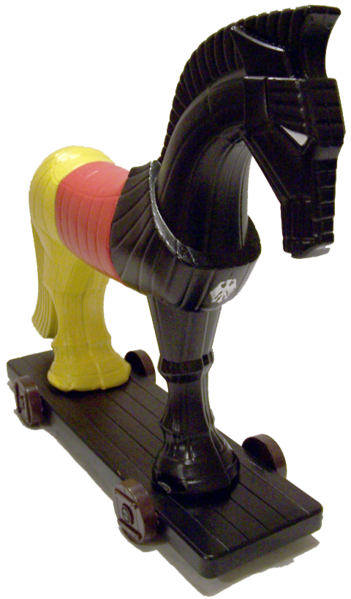
\includegraphics[height=0.7\textheight]{img/trojaner.png}
  \end{figure}
\end{frame}

\begin{frame}
    \frametitle{Chaos Computer Club}
    \begin{center}
	
\includegraphics[height=0.1\textheight]{img/c3d2_logo.png}
    \end{center}
    \begin{itemize}
      \item<1-> Chaos Computer Club Dresden (\url{https://c3d2.de})
      \item<2-> Datenspuren: Herbst 2016 (\url{https://datenspuren.de})
      \item<3-> Podcasts (\url{https://c3d2.de/radio.html})
      \item<4-> Chaos macht Schule (\url{https://c3d2.de/schule.html})
    \end{itemize}
\end{frame}

\begin{frame}
    \frametitle{Bundespräsident Gauck zur NSA-Überwachung}
    \begin{center}
      ``Wir wissen z.B., dass es nicht so ist, wie bei der Stasi und dem KGB, dass es dicke Aktenbände gibt, wo unsere Gesprächsinhalte alle aufgeschrieben und schön abgeheftet sind. Das ist es nicht.''
      (Gauck, 30.06.2013 im ZDF-Sommerinterview)
    \end{center}
\end{frame}

\begin{frame}
    \frametitle{Stasi vs. NSA}
    \begin{center}
      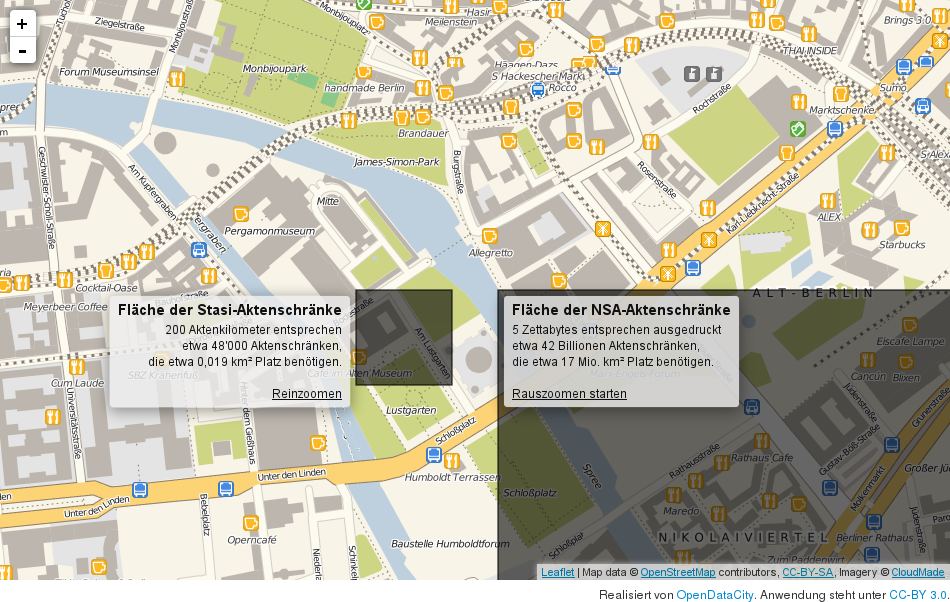
\includegraphics[height=0.7\textheight]{img/akten1.png}
    \end{center}
\end{frame}

\begin{frame}
    \frametitle{Stasi vs. NSA}
    \begin{center}
      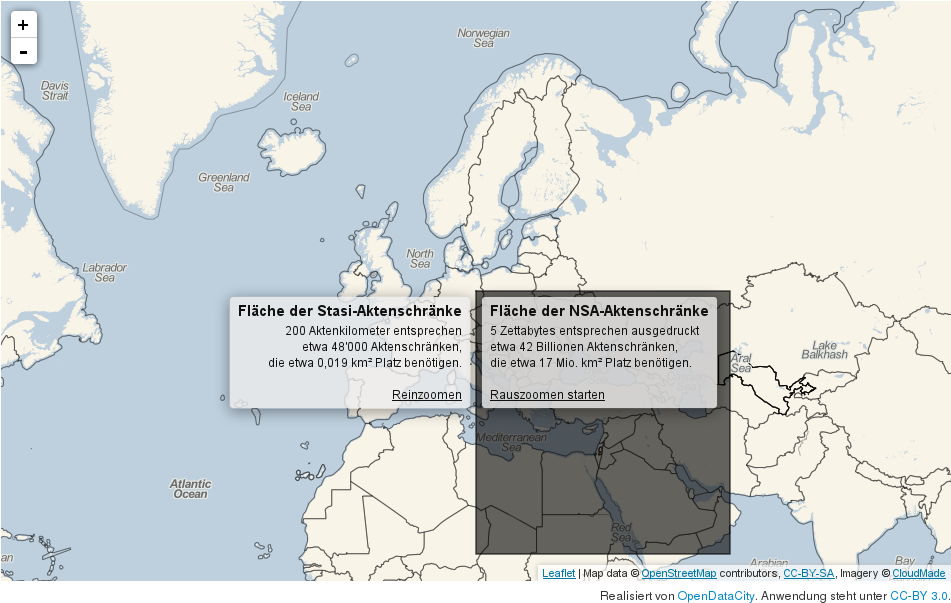
\includegraphics[height=0.7\textheight]{img/akten2.png}
    \end{center}
\end{frame}

\begin{frame}
    \frametitle{``Ich hab ja nichts zu vergergen''}
    \begin{center}
      ``Arguing that you don't care about the right to privacy because you have nothing to hide is no different than saying you don't care about free speech because you have nothing to say. ''
      (Edward Snowden, 21.05.2015 auf Reddit)
    \end{center}
\end{frame}

\begin{frame}
    \frametitle{Samsung vs. 1984}
    \begin{center}
      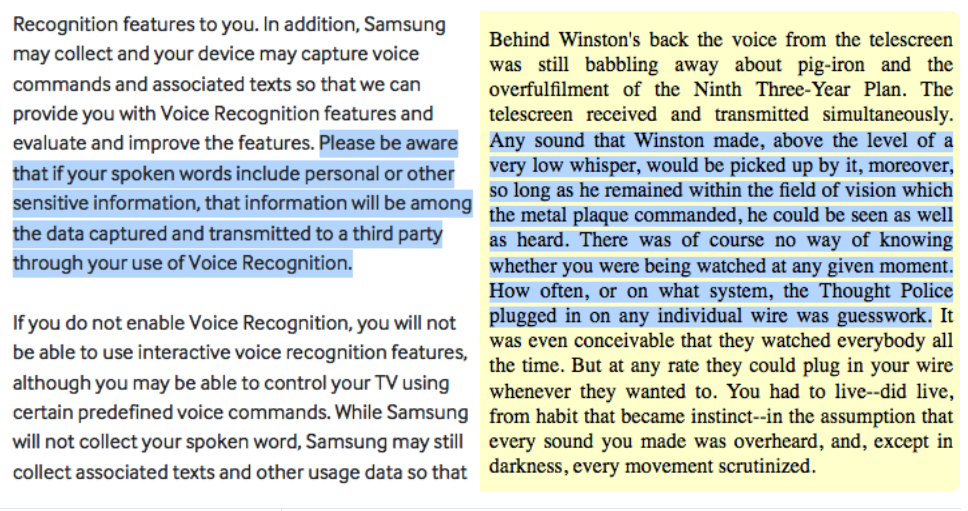
\includegraphics[height=0.7\textheight]{img/samsung-1984.png}
    \end{center}
\end{frame}

\section{Einführung}
\subsection{}

\begin{frame}
    \frametitle{Wie kommunizieren wir im Internet?}
    \begin{center}
      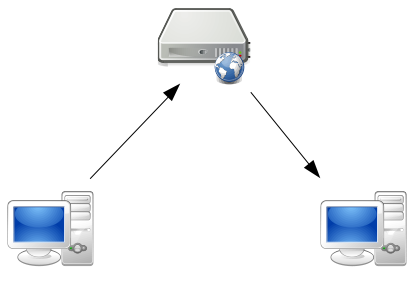
\includegraphics[height=5cm]{img/c-s.png}
    \end{center}
\end{frame}

\begin{frame}
    \frametitle{Server im Rechenzentrum}
    \begin{center}
      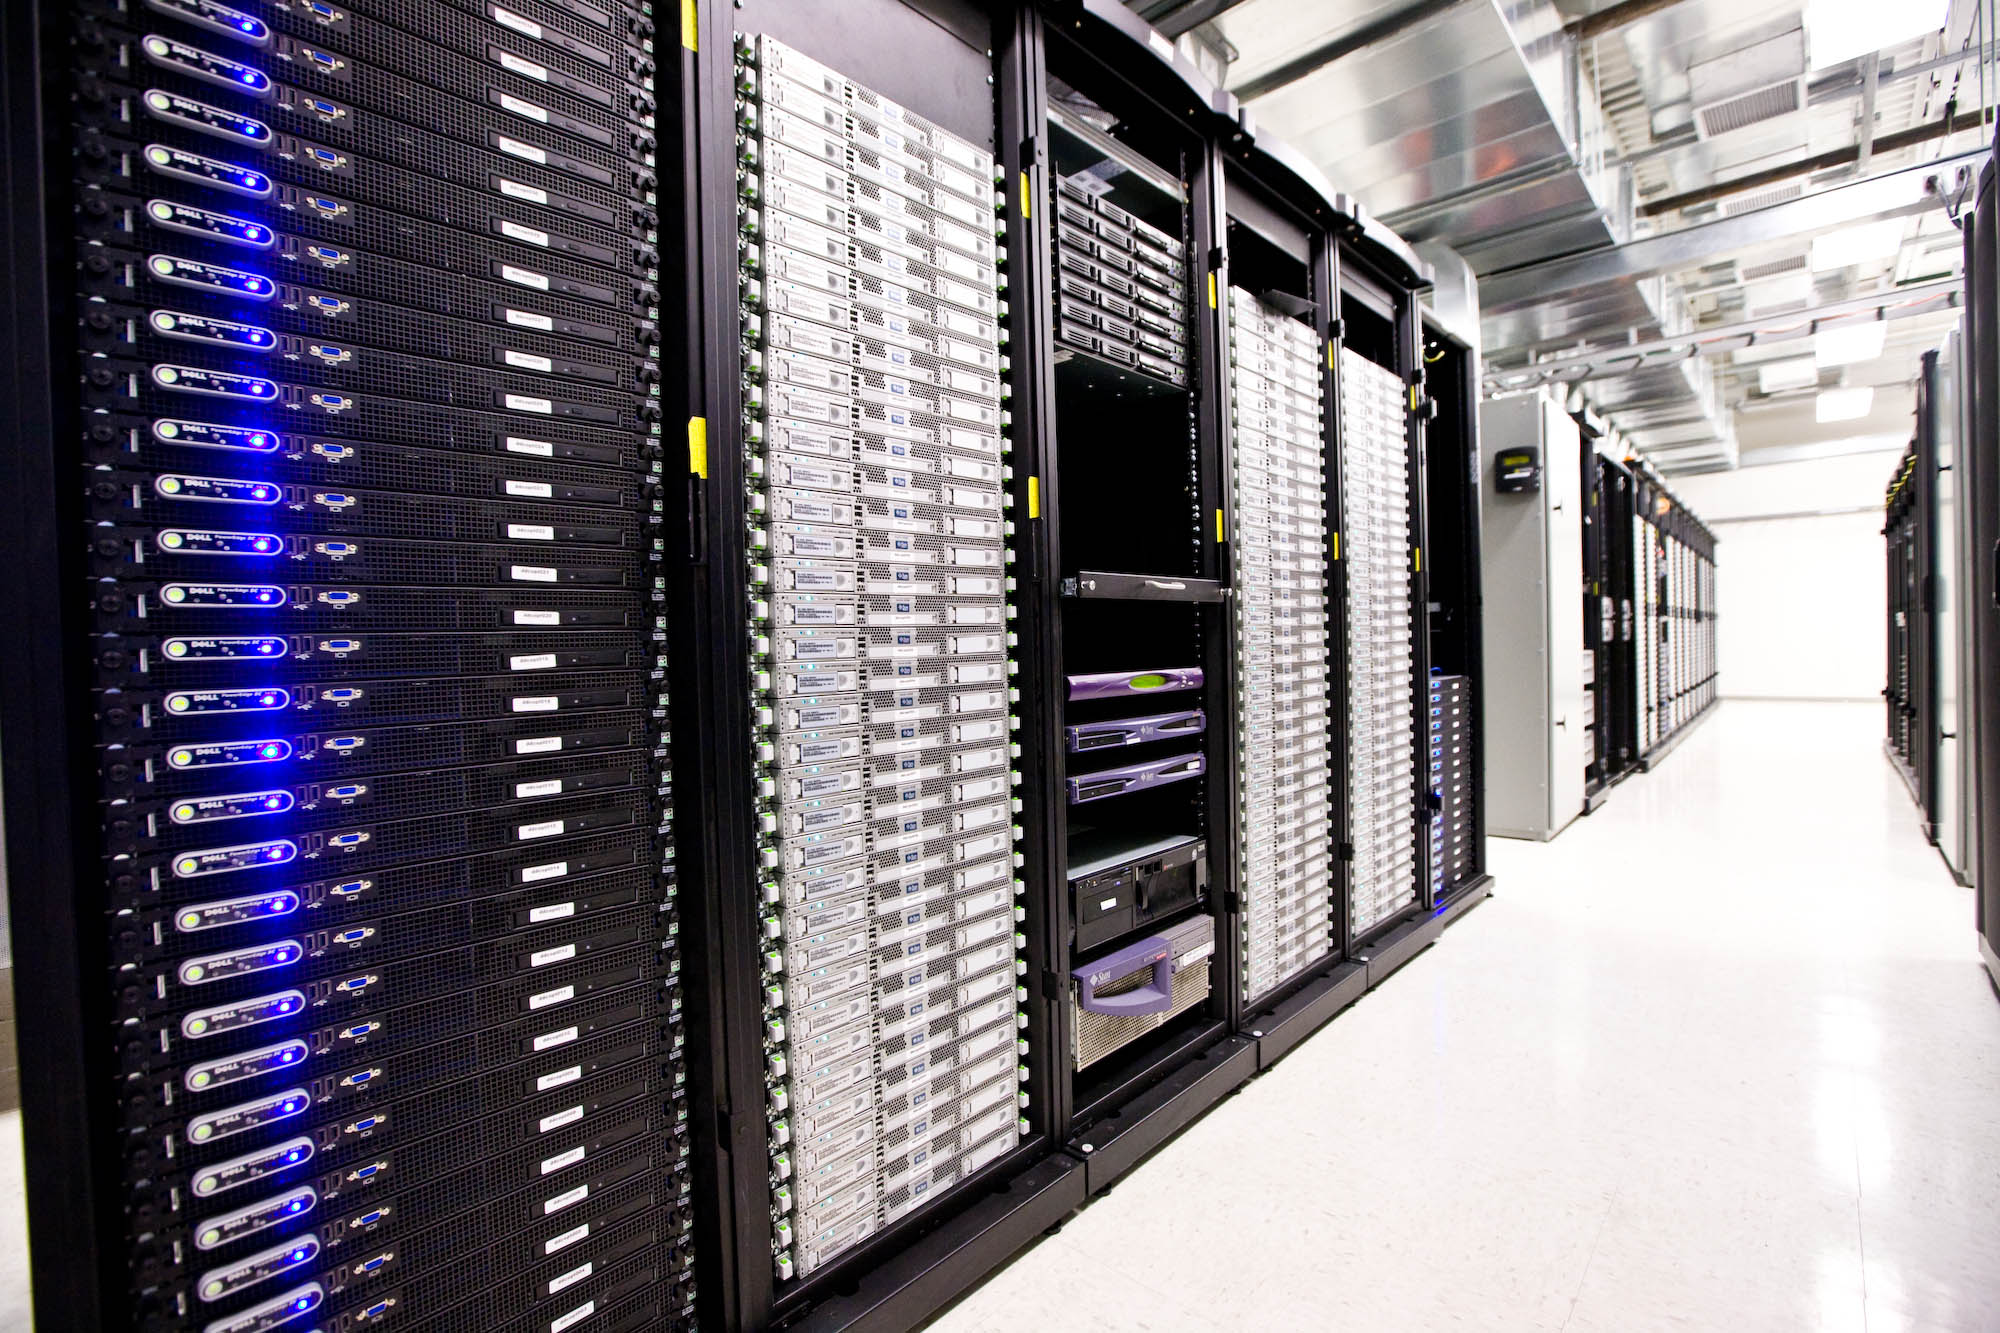
\includegraphics[height=5cm]{img/data_center.jpg}
    \end{center}
\end{frame}

\begin{frame}
    \frametitle{Internetknoten (Router)}
    \begin{center}
      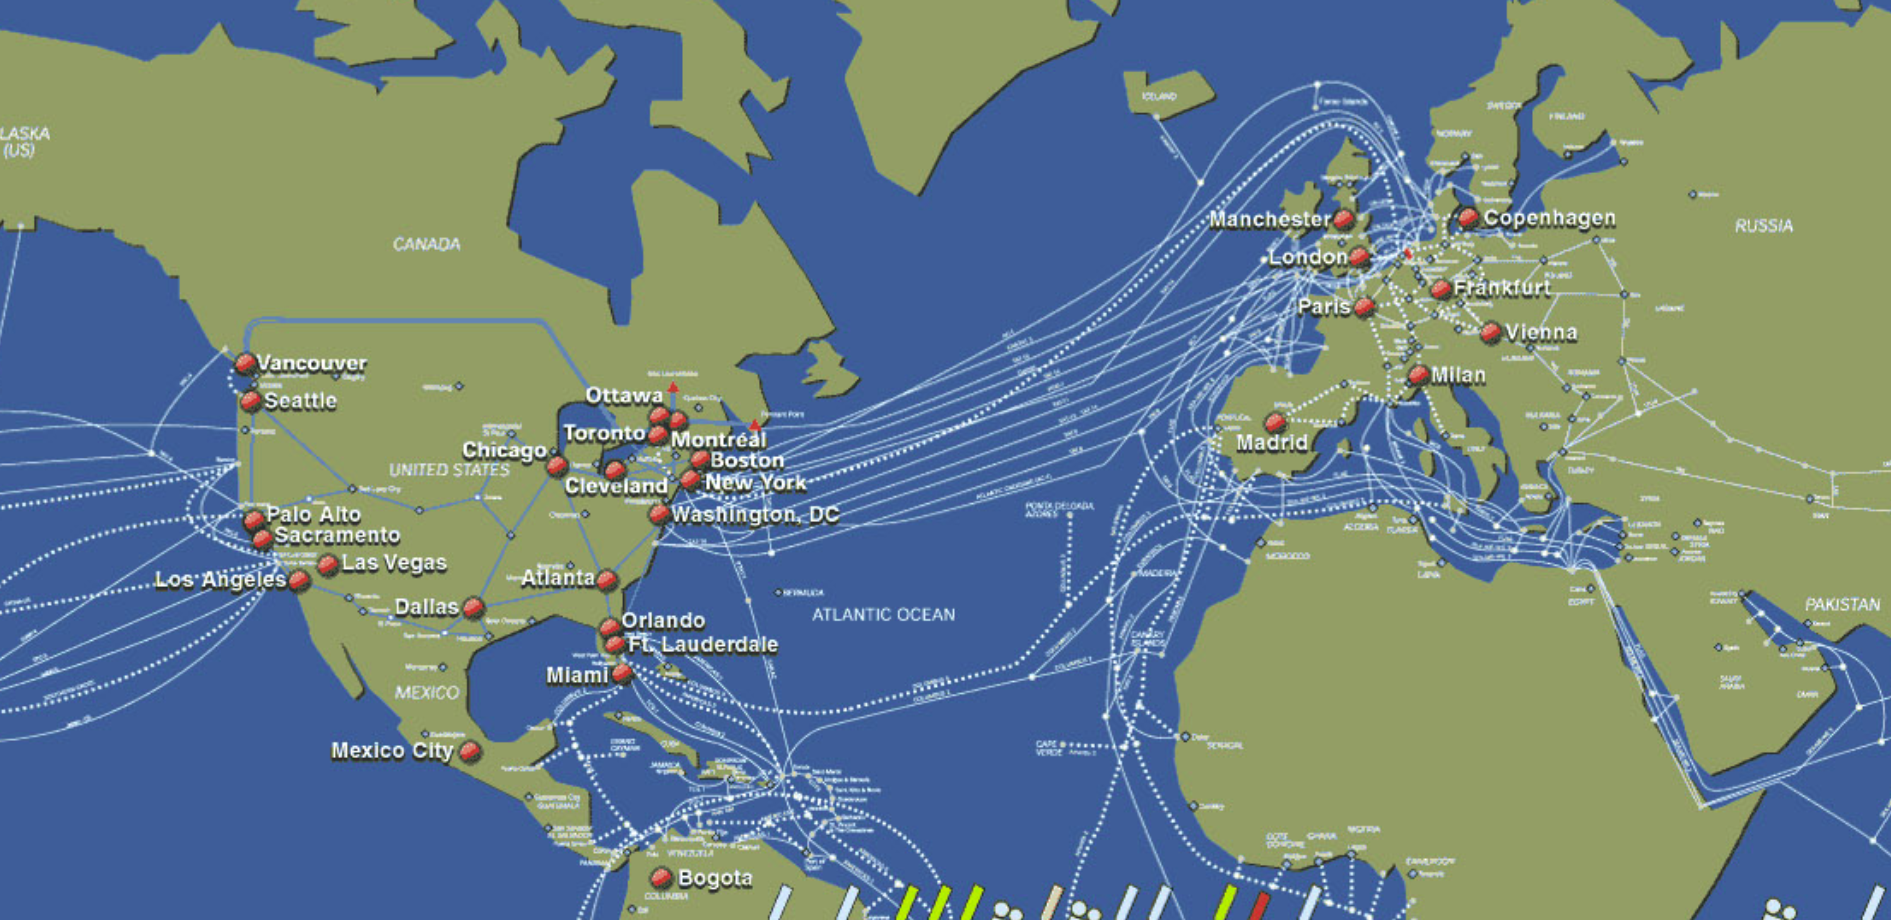
\includegraphics[height=5cm]{img/internet_cable_map.png}
    \end{center}
\end{frame}

\begin{frame}
    \frametitle{Internetknoten (DE-CIX in Frankfurt)}
    \begin{center}
      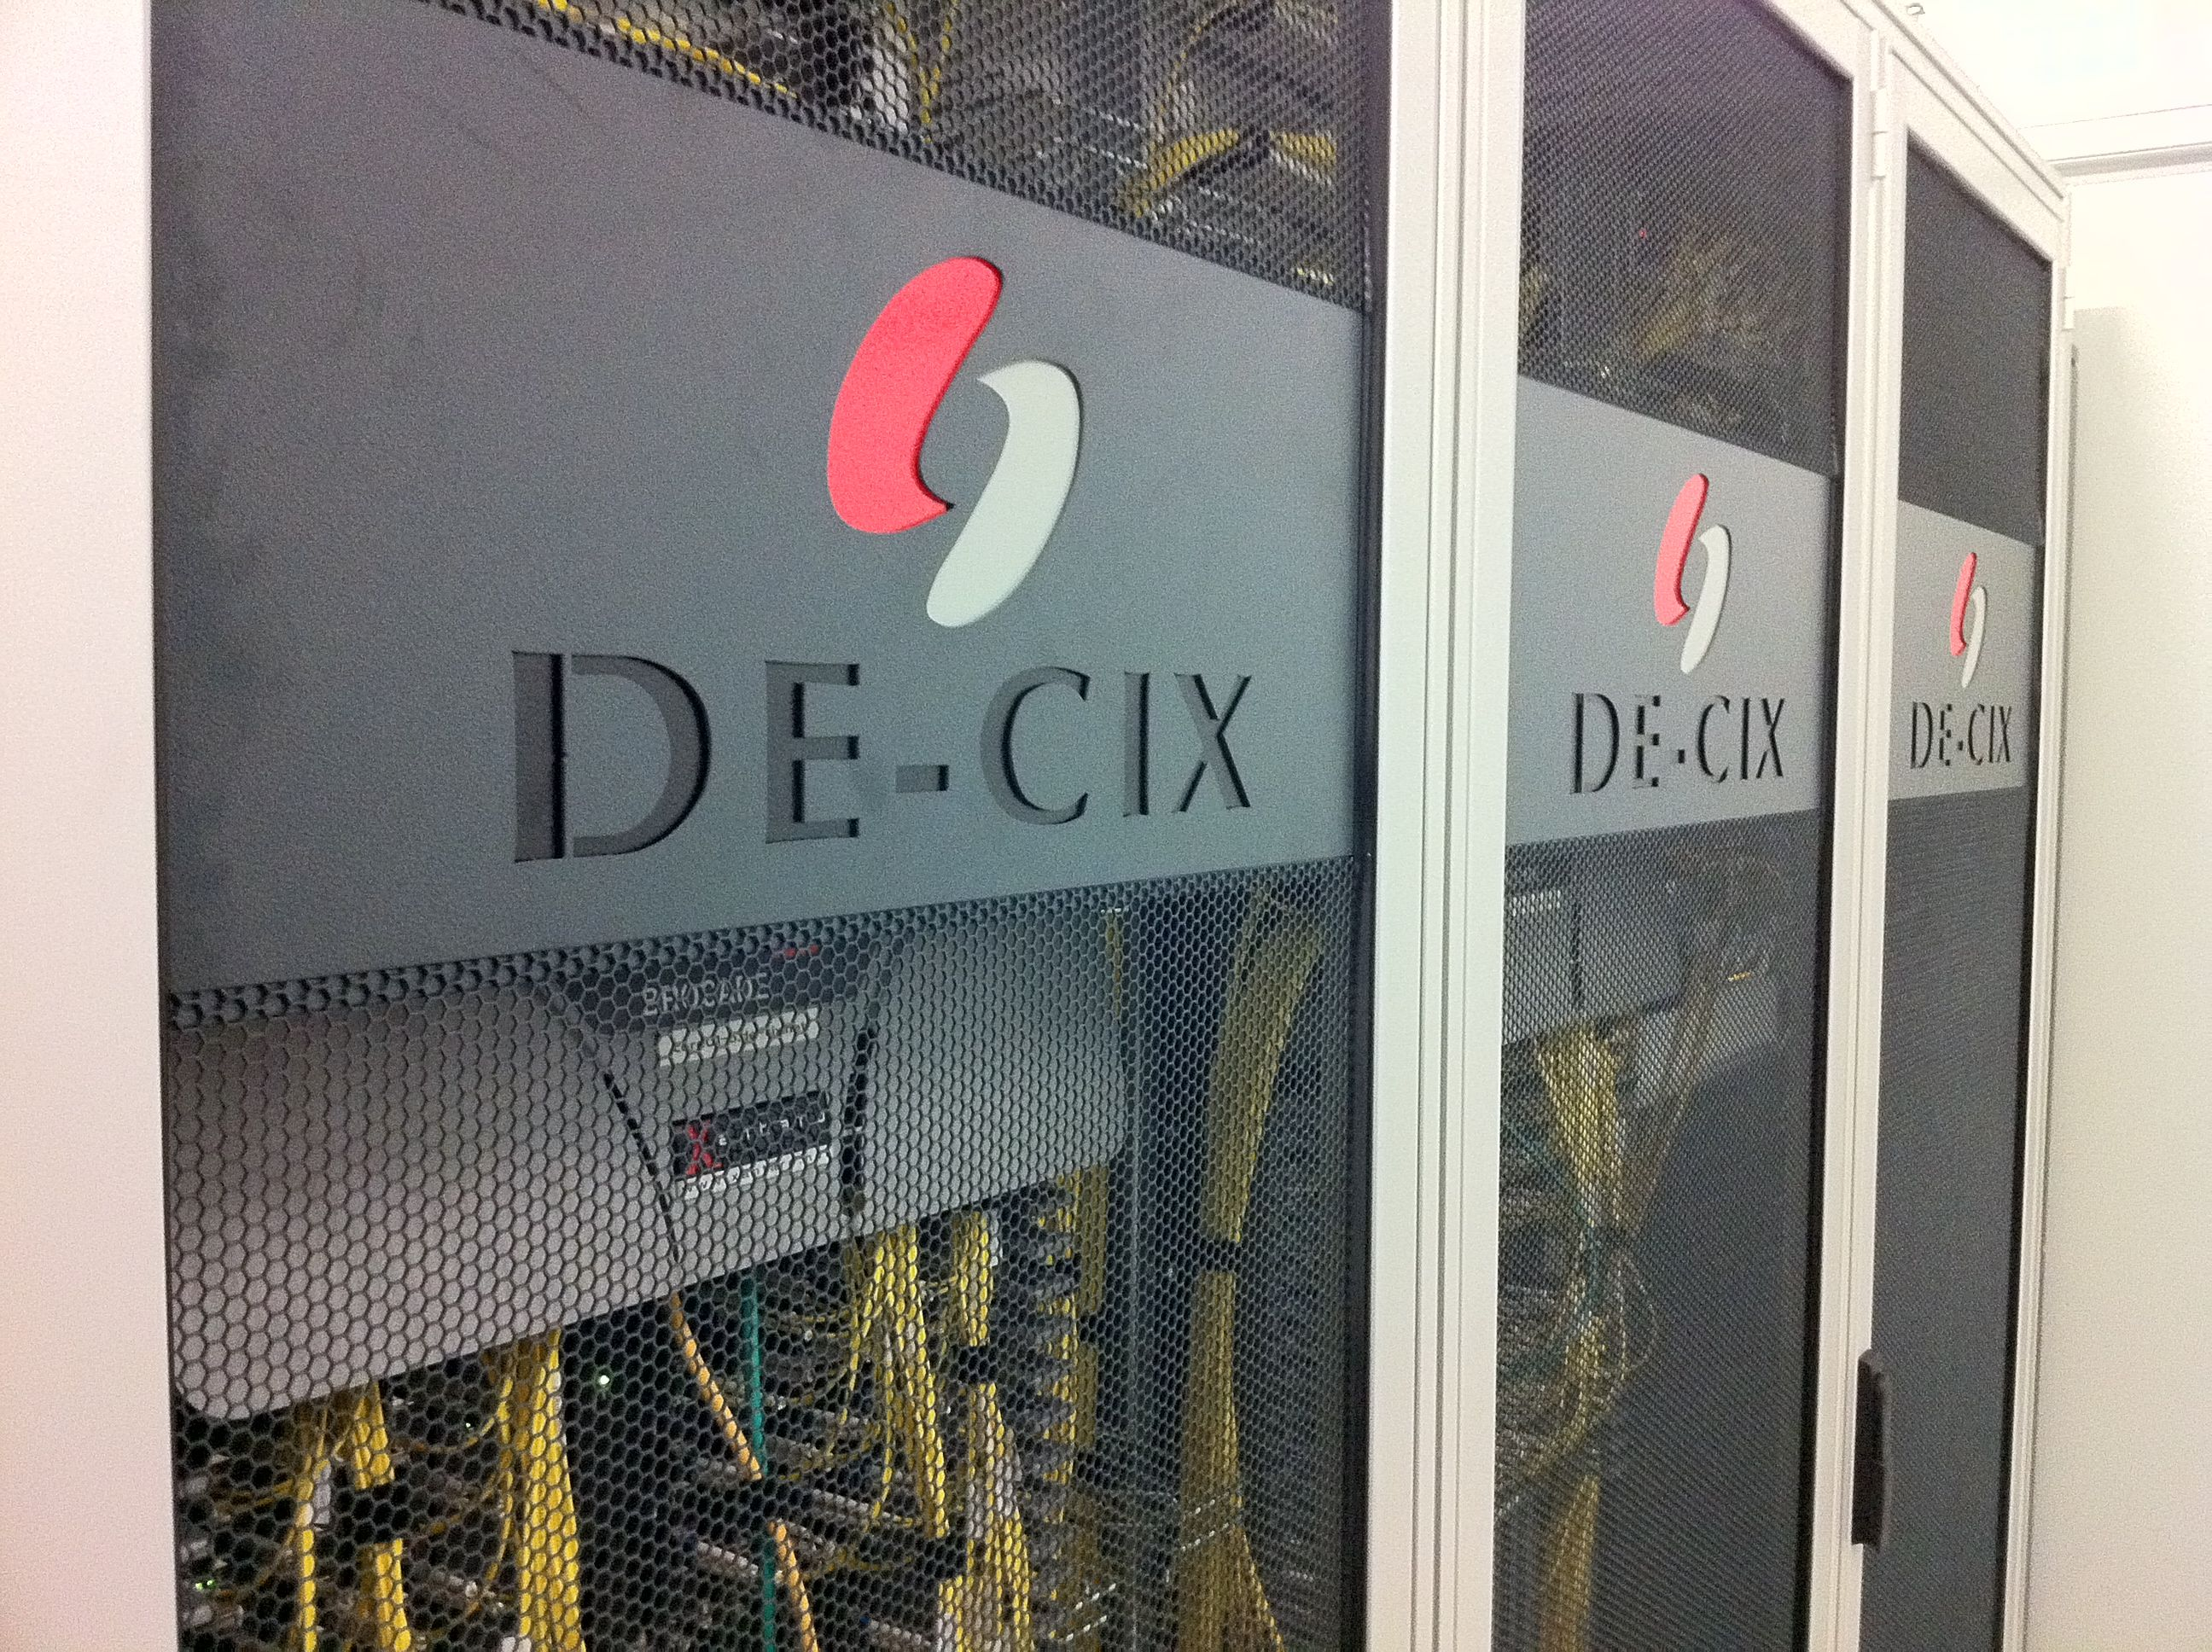
\includegraphics[height=5cm]{img/de_cix.jpg}
      \\{\small \href{https://de.wikipedia.org/wiki/DE-CIX\#/media/File:DE-CIX\_GERMANY\_-\_Switch\_Rack\_\%286218137120\%29.jpg}{Grafik}: \href{https://creativecommons.org/licenses/by-sa/2.0/}{\cc{by-sa} Stefan Funke}}
    \end{center}
\end{frame}

\begin{frame}
    \frametitle{Was ist zu schützen?}
    \begin{center}
      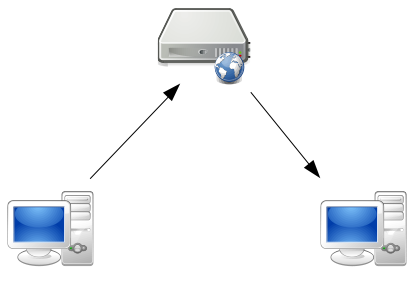
\includegraphics[height=5cm]{img/c-s.png}
    \end{center}
\end{frame}

\section{Geräte}
\subsection{}

\begin{frame}
  \frametitle{Backdoors}
  \begin{center}
    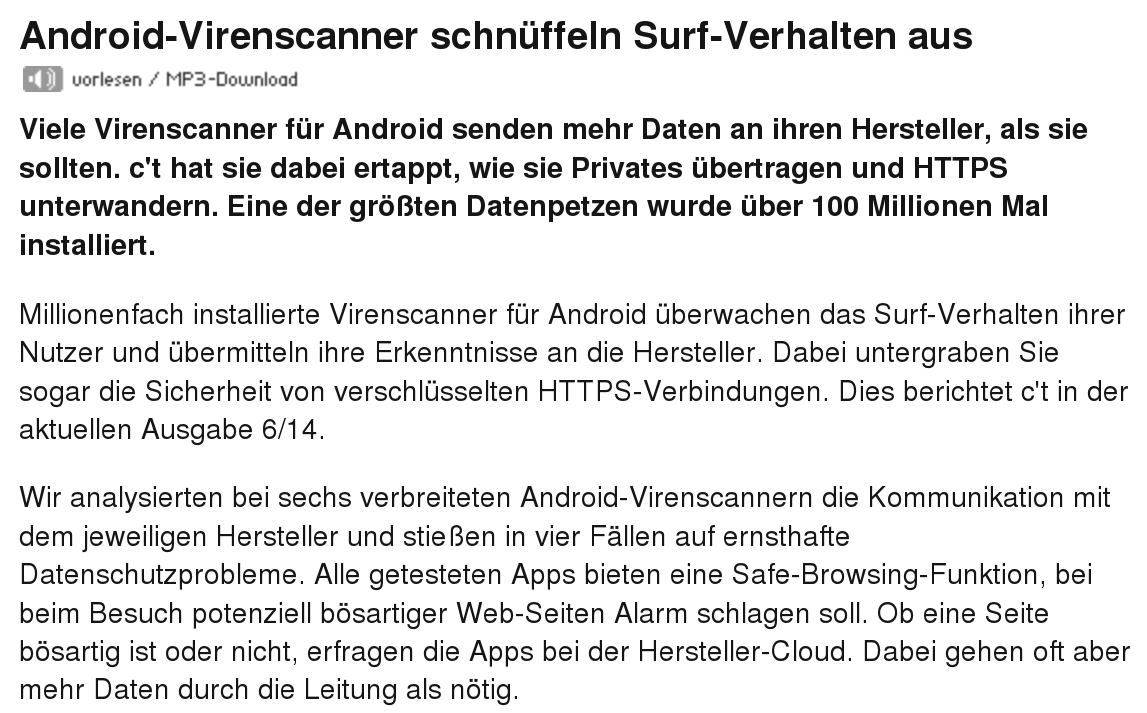
\includegraphics[width=10cm]{img/backdoor-av}
  \par\end{center}
\end{frame}

\begin{frame}
    \frametitle{Unerwünschte Funktionalität}
    \begin{center}
      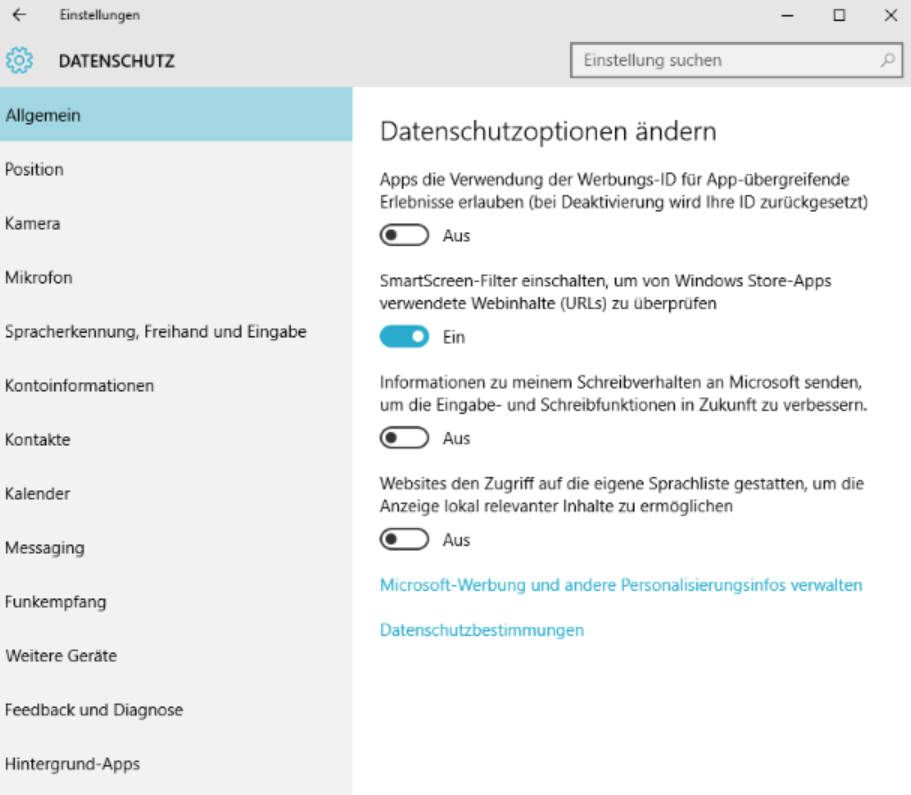
\includegraphics[width=0.7\textwidth]{img/windows10.png}
    \end{center}
\end{frame}

\begin{frame}
  \frametitle{Unerwünschte Funktionalität}
  \begin{center}
    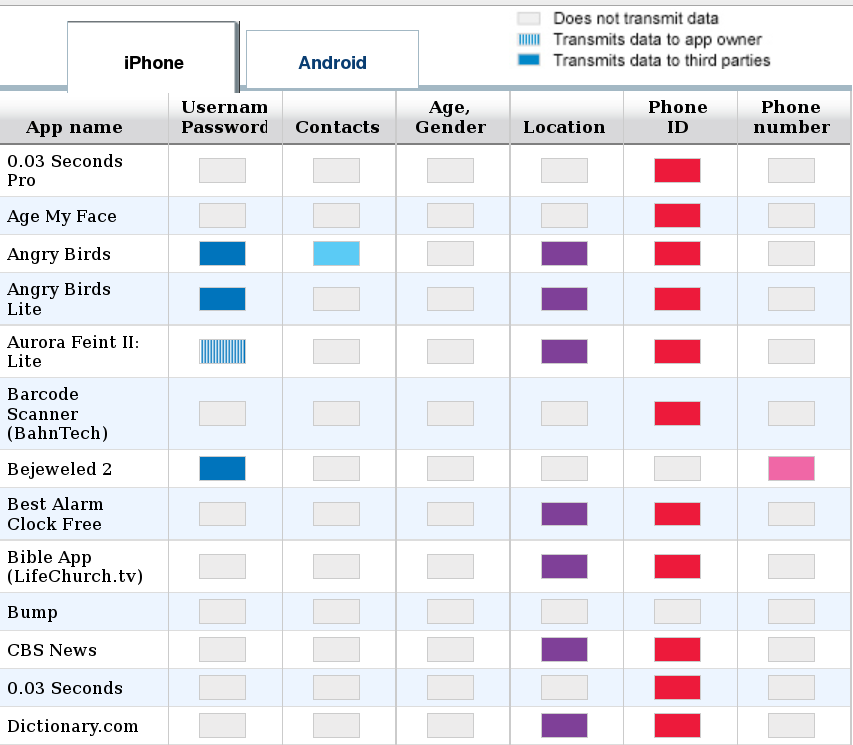
\includegraphics[width=7cm]{img/backdoor-apps}
  \par\end{center}
\end{frame}

\begin{frame}
  \frametitle{Unerwünschte Funktionalität}
  \begin{center}
    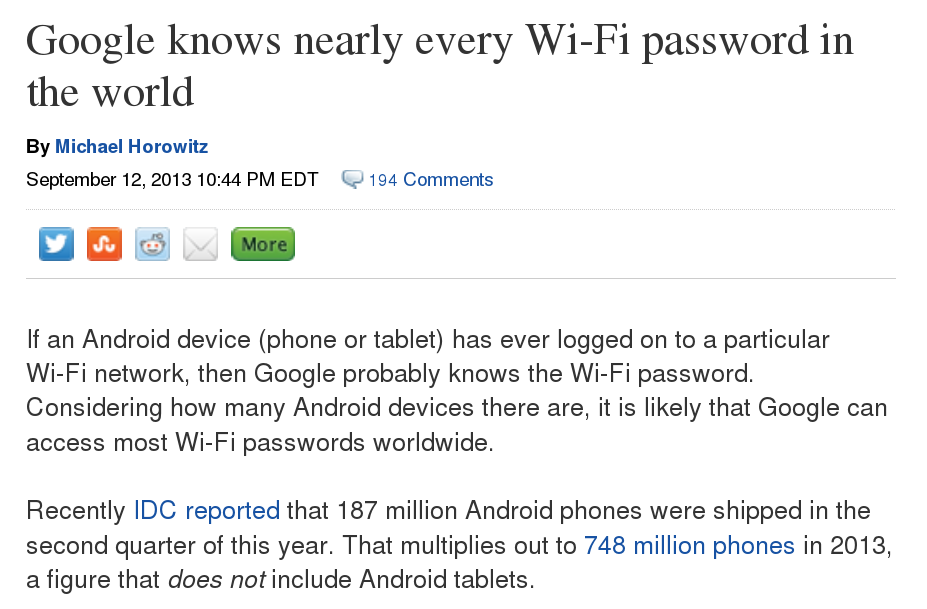
\includegraphics[width=10cm]{img/backdoor-android}
  \par\end{center}
\end{frame}

\begin{frame}
    \frametitle{Wie schütze ich meine Geräte?}
    \begin{itemize}
      \item Rechte von Applikationen einschränken (Permissions, Firewall)
      \item Aktuelle und vertrauenswürdige Software
    \end{itemize}
\end{frame}

\begin{frame}{Permissions}
  \begin{columns}
    \column{5.5cm}
    \footnotesize

    \textbf{Android}\\
    Einstellungen -> Apps -> Appname -> Berechtigungen ändern\\
    \vspace{0.2cm}
    Einstellungen -> Apps -> Zahnrad -> Appberechtigungen\\
    \vspace{0.5cm}

    \textbf{iOS}\\
    Einstellungen -> Privatsphäre -> Berechtigungsname\\
    \vspace{0.5cm}

    In den neuesten Versionen: Entscheidung bei erster Benutzung

    \column{5cm}

    \begin{center}
      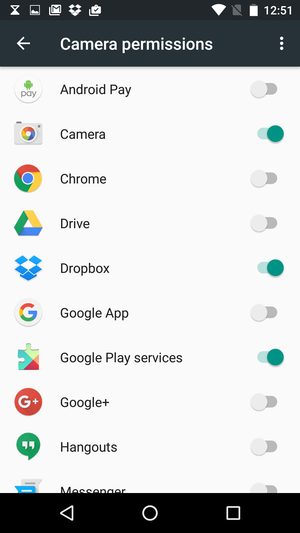
\includegraphics[width=3.5cm]{img/permissions-android.png}
    \par\end{center}
  \end{columns}
\end{frame}

\begin{frame}
    \frametitle{Vertrauenswürdige Software?}
    \begin{center}\Large
        Einer Software, die nicht quelloffen ist, kann man nicht vertrauen
    \end{center}
\end{frame}

\begin{frame}
  \frametitle{Kompilierung von Software}
  \begin{center}
    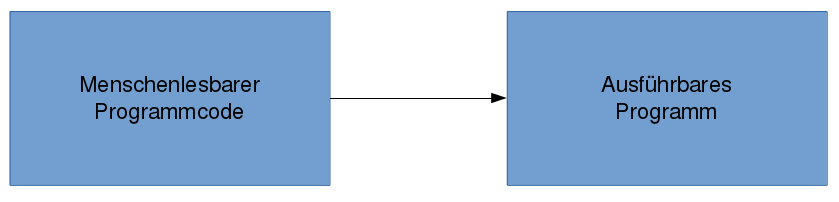
\includegraphics[width=10cm]{img/compilation-process}
  \par\end{center}
\end{frame}

\begin{frame}{Das GNU Projekt}
  \begin{columns}
    \column{6cm}

    \begin{itemize}
      \item Begonnen von Richard Stallman im Jahr 1984 
      \item Gründung der Free Software Foundation im Jahr 1985 
    \end{itemize}

    \column{7cm}

    \begin{center}
      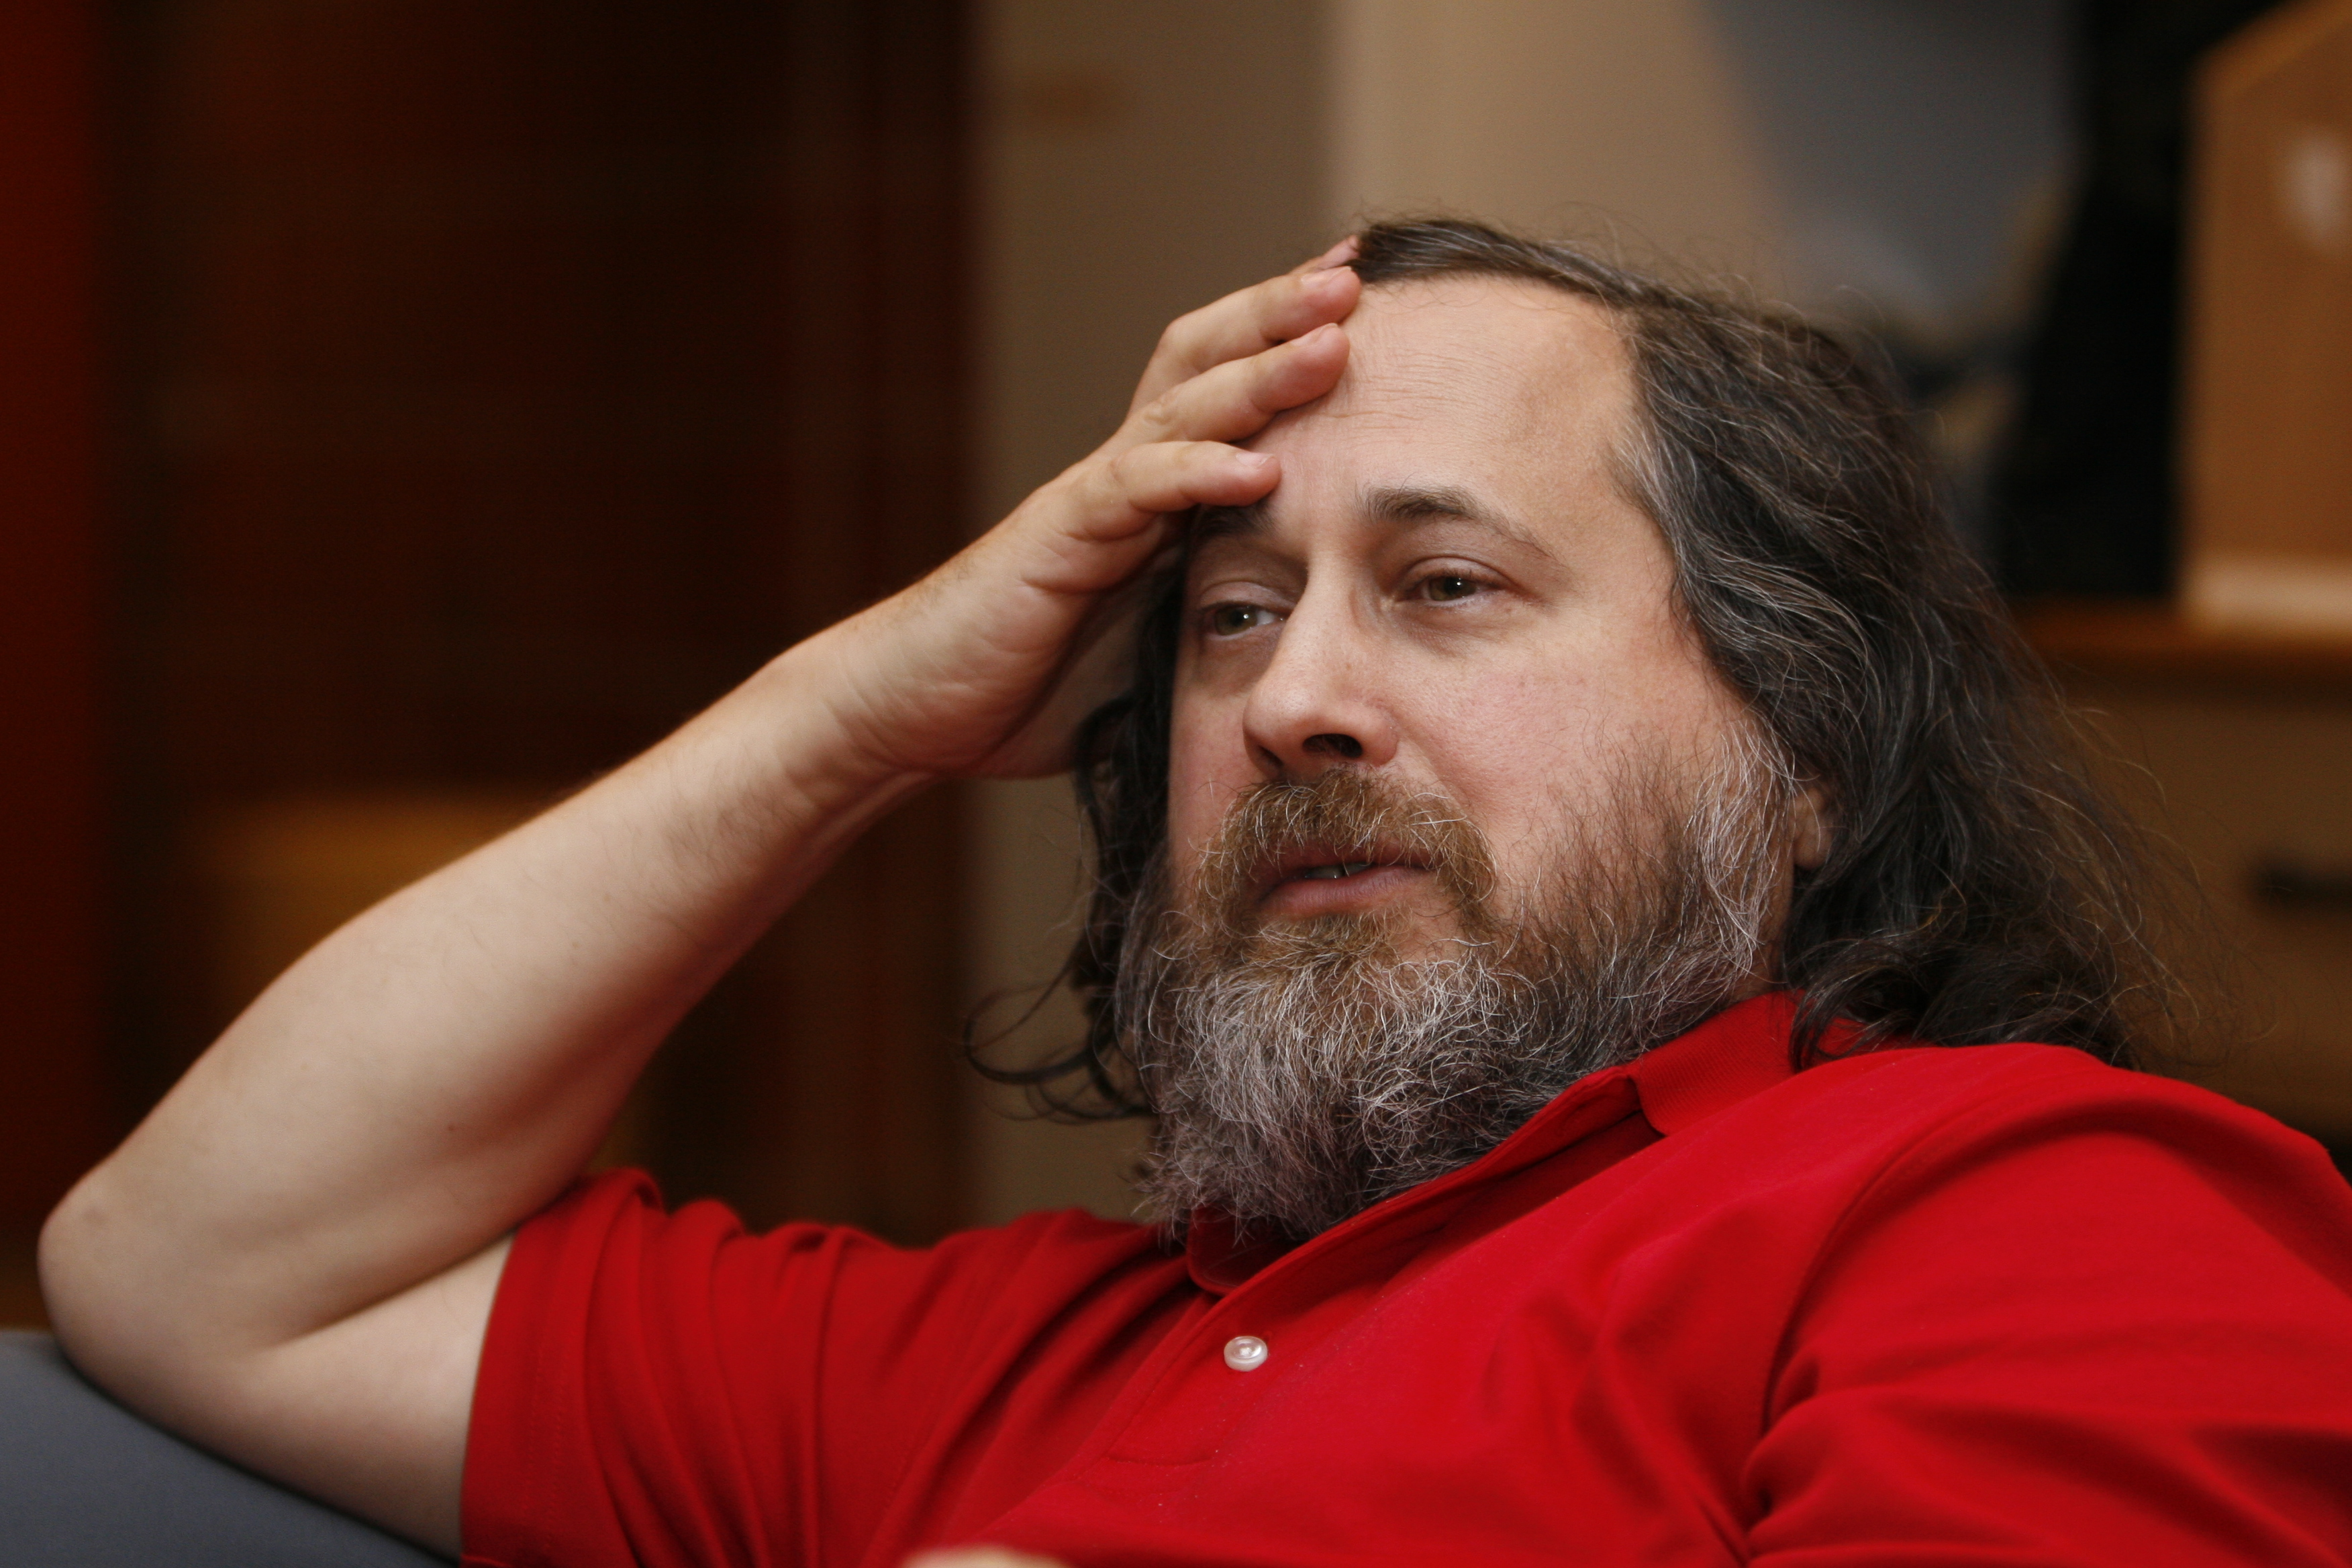
\includegraphics[width=4.5cm]{img/stallman}
    \par\end{center}

    \begin{center}
      
\includegraphics[width=5cm]{img/logo-fsf}
    \par\end{center}
  \end{columns}
\end{frame}

\begin{frame}
  \frametitle{Freie Software auf Computern}
    \begin{columns}
        \begin{column}{5cm}
            \begin{center}
                
\includegraphics[height=0.2\textheight]{img/firefox.png} \\
                Firefox \\
                \vspace{0.1\textheight}
                
\includegraphics[height=0.2\textheight]{img/libreoffice.jpg}\\
                LibreOffice
            \end{center}
        \end{column}
        \begin{column}{5cm}
            \begin{center}
                
\includegraphics[height=0.2\textheight]{img/thunderbird.png} \\
                Thunderbird \\
                \vspace{0.1\textheight}
                
\includegraphics[height=0.2\textheight]{img/vlc.png}\\
                VLC Media Player
            \end{center}
        \end{column}
    \end{columns}
\end{frame}

\begin{frame}{Freie Software auf dem Smartphone}
  \begin{columns}
    \column{6.5cm}

    \textbf{F-Droid}\\
    Android-Appstore für freie Software

    \vspace{0.5cm}

    \textbf{iOS Open Source Apps}\\
    \url{https://github.com/dkhamsing/open-source-ios-apps}

    \column{5cm}

    \begin{center}
      
\includegraphics[width=2cm]{img/F-Droid_Logo_2}
    \par\end{center}
    \begin{center}
    \par\end{center}
  \end{columns}
\end{frame}

\begin{frame}{Cyanogenmod, Replicant}
  \begin{columns}
    \column{6cm}
    \begin{itemize}
      \item basiert auf Open Source Teil von Android
      \item ersetzt teilweise die proprietären Apps durch freie
      \item \textbf{Problem:} Verlust der Garantie bei Installation
    \end{itemize}
    \column{5cm}
    \begin{center}
      
\includegraphics[width=4cm]{img/cyanogenmod.png}
    \par\end{center}
  \end{columns}
\end{frame}

\begin{frame}
  \frametitle{Ubuntu Phone, Sailfish OS}
    \begin{center}
      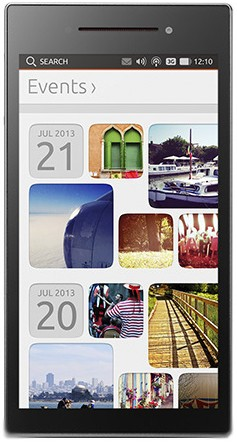
\includegraphics[height=6cm]{img/ubuntuphone.jpg}
      \hspace{0.5cm}
      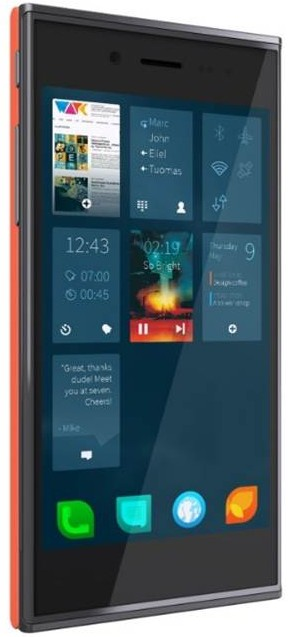
\includegraphics[height=6cm]{img/sailfishos.jpg}
    \end{center}
\end{frame}

\begin{frame}{Geräteverschlüsselung auf Computern}
  \begin{columns}
    \column{4cm}
    \footnotesize

    \textbf{Linux}\\
    Standardmäßig vorhanden, muss beim Installieren ausgewählt werden
    \vspace{0.5cm}

    \textbf{Windows}\\
    TrueCrypt, Veracrypt
    \vspace{0.5cm}

    \textbf{Mac}\\
    FileVault, muss beim Installieren ausgewählt werden
    \vspace{0.5cm}
    \column{5cm}

    \begin{center}
      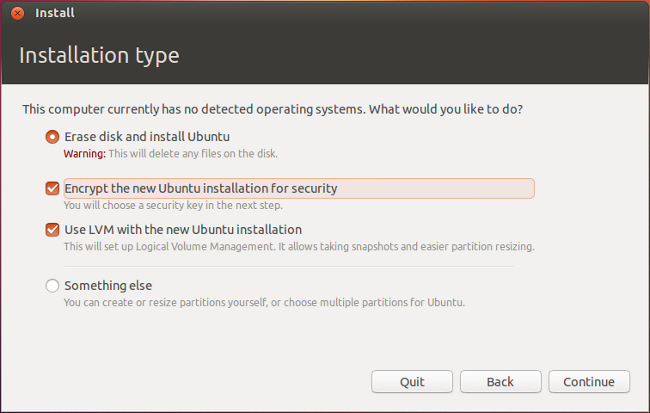
\includegraphics[width=5cm]{img/encryption-ubuntu.png}
    \par\end{center}
  \end{columns}
\end{frame}

\begin{frame}{Geräteverschlüsselung auf Smartphones}
  \begin{columns}
    \column{5.5cm}
    \footnotesize

    \textbf{Android}\\
    Standard ab 6.0
    Einstellungen -> Sicherheit -> Telefon verschlüsseln\\
    \vspace{0.5cm}

    \textbf{iOS}\\
    Standard\\
    \vspace{0.5cm}
    \textbf{wichtig:} gute PIN/Muster

    \column{5cm}

    \begin{center}
      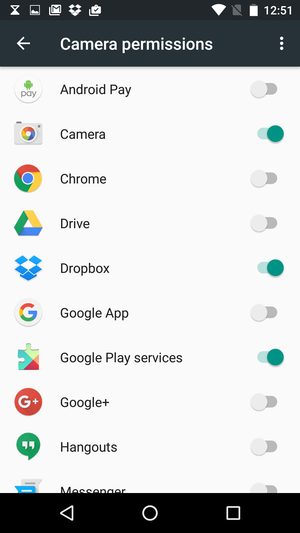
\includegraphics[width=3.5cm]{img/permissions-android.png}
    \par\end{center}
  \end{columns}
\end{frame}

\begin{frame}
    \frametitle{Was ist zu schützen?}
    \begin{center}
      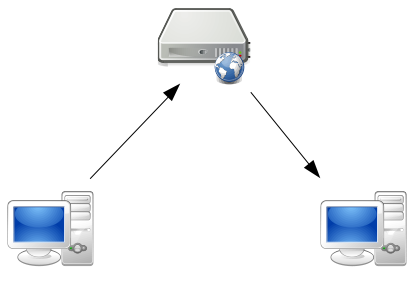
\includegraphics[height=5cm]{img/c-s.png}
    \end{center}
\end{frame}

\section{Inhalte}
\subsection{}

\begin{frame}
    \frametitle{Angreifer im eigenen Netz}
    \begin{center}
      
\includegraphics[height=0.5\textheight]{img/wifi.png}
    \end{center}
\end{frame}

\begin{frame}
    \frametitle{Transportwegverschlüsselung}
      SSL = Secure Socket Layer / TLS = Transport Layer Security
    \vfill
    \begin{center}
      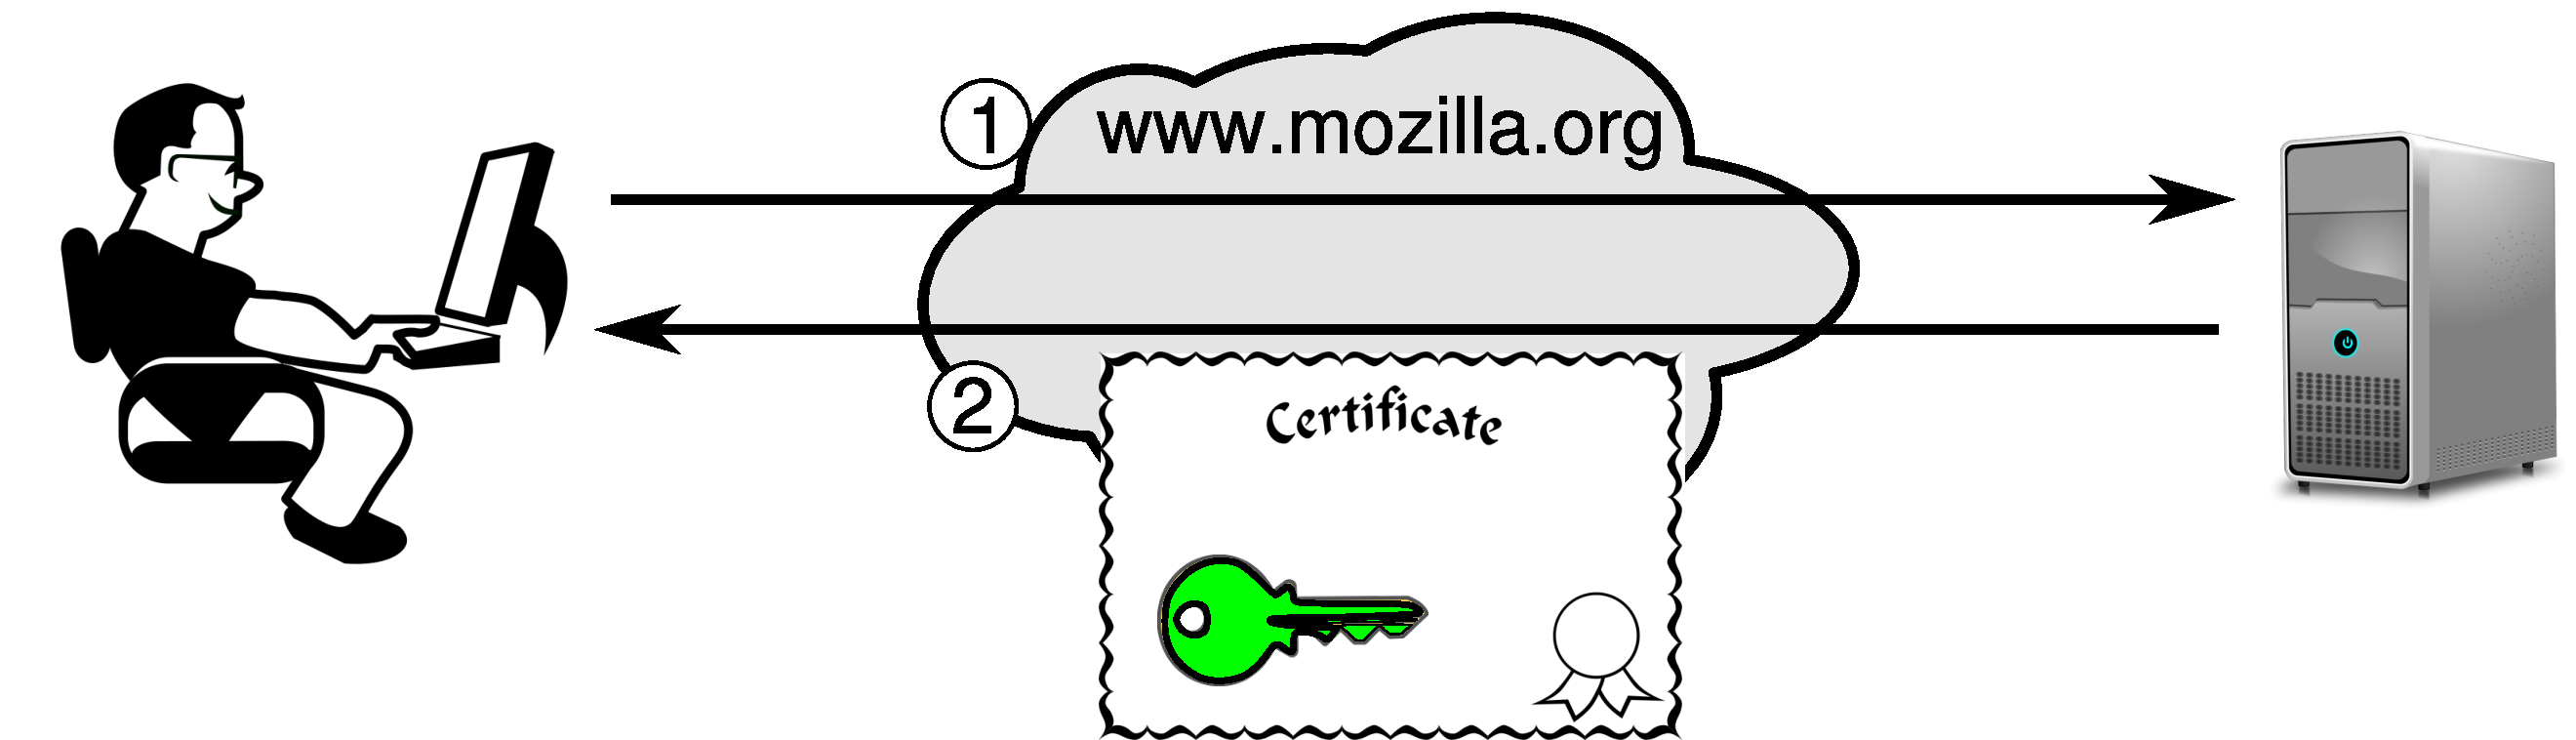
\includegraphics[width=0.8\textwidth]{img/tls.pdf}
    \end{center}
\end{frame}

\begin{frame}
    \frametitle{SSL im Browser}
    \begin{center}
	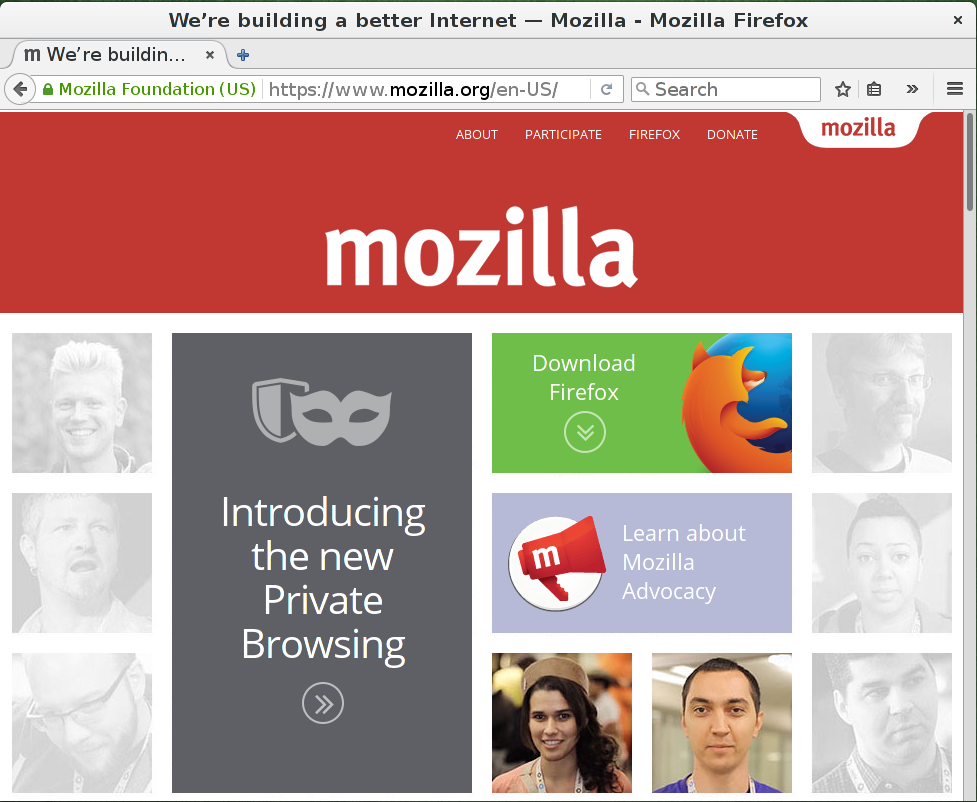
\includegraphics[height=0.7\textheight]{img/ssl_special.png}
    \end{center}
\end{frame}

\begin{frame}
    \frametitle{Ungültiges Zertifikat}
    \begin{center}
	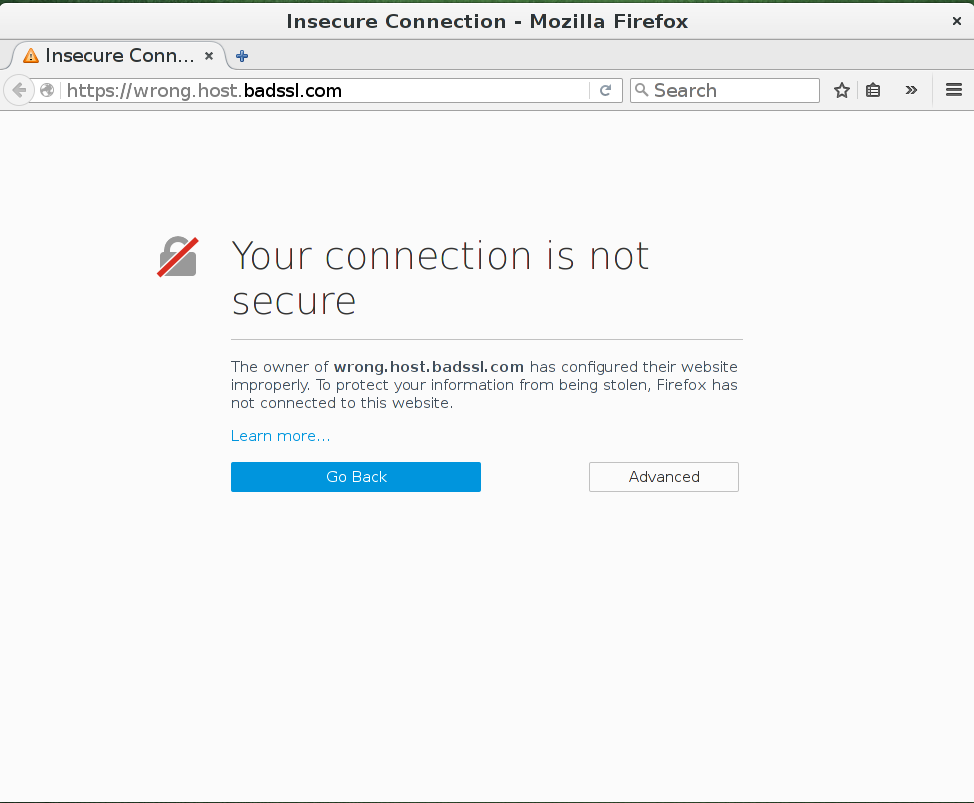
\includegraphics[height=0.7\textheight]{img/ssl_badcert.png}
    \end{center}
\end{frame}

\begin{frame}
    \frametitle{Was ist zu schützen?}
    \begin{center}
      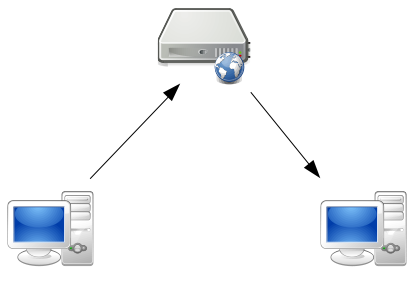
\includegraphics[height=5cm]{img/c-s.png}
    \end{center}
\end{frame}

\begin{frame}
    \frametitle{Informationsleaks}
    \begin{center}
      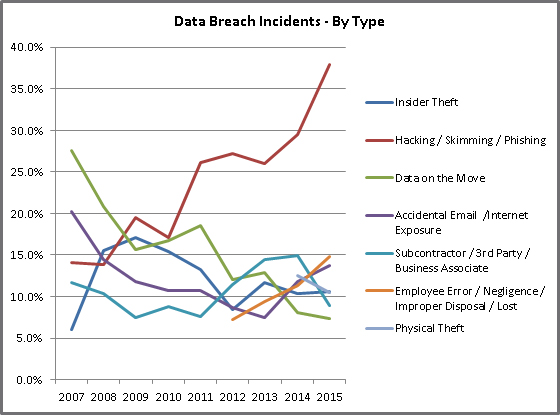
\includegraphics[height=0.7\textheight]{img/databreaches.jpg}\\
      http://www.idtheftcenter.org/ITRC-Surveys-Studies/2015databreaches.html
    \end{center}
\end{frame}

\begin{frame}
  \frametitle{Ende-zu-Ende-Verschlüsselung}
  \begin{itemize}
    \item<1-> GPG für E-Mails
    \item<2-> OTR/OMEMO für Jabber:
      \begin{itemize}
        \item Pidgin für Linux und Windows
        \item Conversations oder ChatSecure für Android
        \item Adium für Mac, ChatSecure für iOS
      \end{itemize}
    \item<3-> palava.tv, talky.io, Tox, Linphone für Videotelefonie
    \item<4-> Signal
  \end{itemize}
\end{frame}

\begin{frame}
  \frametitle{Jabber: Conversations, ChatSecure}
    \begin{center}
      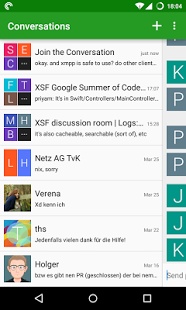
\includegraphics[height=6cm]{img/conversations.png}
      \hspace{0.5cm}
      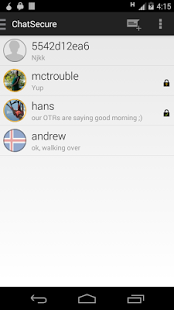
\includegraphics[height=6cm]{img/chatsecure.png}
    \end{center}
    \url{https://xmpp.net/directory.php}
\end{frame}

\begin{frame}
  \frametitle{Signal}
    \begin{center}
      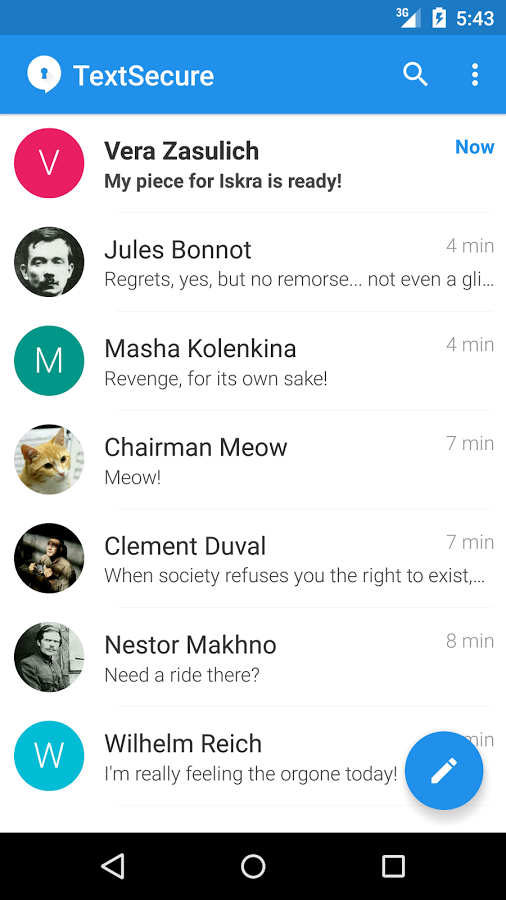
\includegraphics[height=6cm]{img/signal1.png}
      \hspace{0.5cm}
      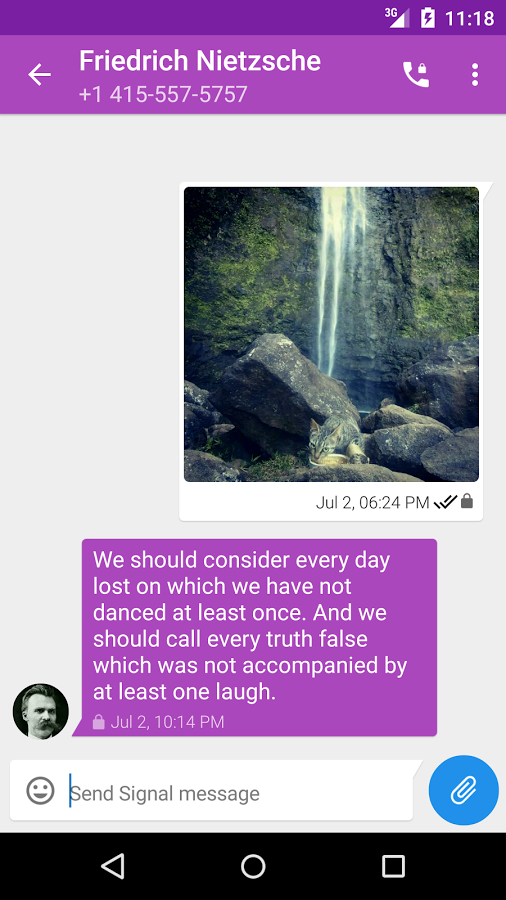
\includegraphics[height=6cm]{img/signal2.png}
    \end{center}
\end{frame}

\begin{frame}
  \frametitle{Vergleich Messenger}
  \small
  \begin{tabular}{|c|c|c|c|c|c|}
    \hline
                      & Whatsapp            & Threema             & Telegram              & Signal                & Jabber              \\
    \hline
    Verschlüsselung   & \cellcolor{orange}  & \cellcolor{yellow}  & \cellcolor{orange}    & \cellcolor{green}     & \cellcolor{green}   \\
    \hline
    Vertrauensw.      & \cellcolor{red}     & \cellcolor{yellow}  & \cellcolor{orange}    & \cellcolor{green}     & \cellcolor{green}   \\
    \hline
    Dezentr.          & \cellcolor{red}     & \cellcolor{red}     & \cellcolor{red}       & \cellcolor{orange}    & \cellcolor{green}   \\
    \hline
    Open Source       & \cellcolor{red}     & \cellcolor{red}     & \cellcolor{yellow}    & \cellcolor{green}     & \cellcolor{green}   \\
    \hline
    Mobileignung      & \cellcolor{green}   & \cellcolor{green}   & \cellcolor{green}     & \cellcolor{green}     & \cellcolor{yellow}  \\
    \hline
  \end{tabular}
\end{frame}

\section{Dezentrale Dienste}
\subsection{}

\begin{frame}
  \frametitle{Dezentrale Dienste}
    \begin{columns}
        \begin{column}{5cm}
            \begin{center}
                
\includegraphics[height=0.2\textheight]{img/mail.pdf} \\
                E-Mail \\
                \vspace{1cm}
                
\includegraphics[height=0.2\textheight]{img/jabber.png}
            \end{center}
        \end{column}
        \begin{column}{5cm}
            \begin{center}
                
\includegraphics[height=0.2\textheight]{img/owncloud.png} \\
                \vspace{1cm}
                
\includegraphics[width=0.8\textwidth]{img/sandstorm.png}
            \end{center}
        \end{column}
    \end{columns}
\end{frame}

\begin{frame}{Owncloud}
  \begin{columns}
    \column{4cm}
    \footnotesize

    Plattformübergreifende Synchronisierung von Dateien, Dokumenten, Kalendern, Kontakten, Notizen und News.

    \column{6cm}

    \begin{center}
      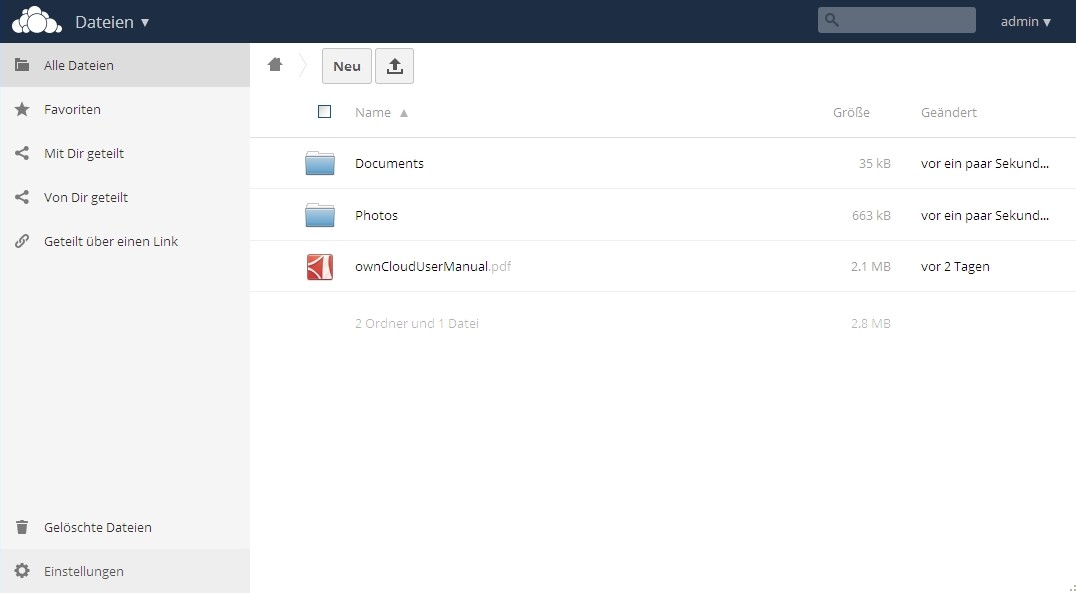
\includegraphics[width=6cm]{img/owncloud-screenshot.jpg}
    \par\end{center}
  \end{columns}
\end{frame}

\begin{frame}{Owncloud als Ersatz für Dropbox}
  \begin{center}
    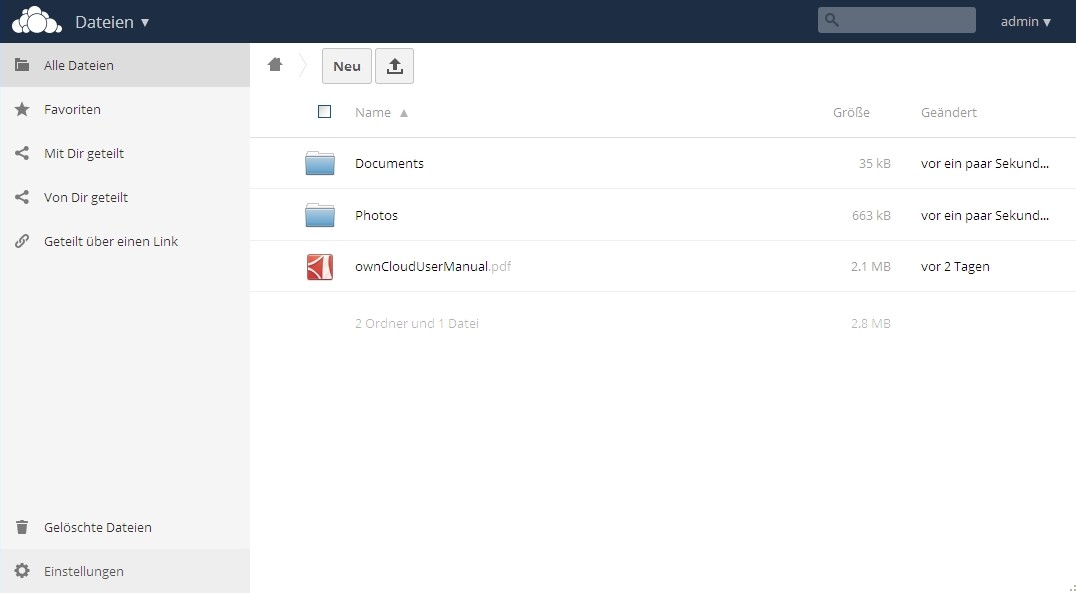
\includegraphics[width=9cm]{img/owncloud-screenshot.jpg}
  \end{center}
\end{frame}

\begin{frame}{Owncloud als Ersatz für Google/Apple-Sync}
  \begin{center}
    \includegraphics[width=9cm]{img/owncloud-calendar.png}
  \end{center}
\end{frame}

\begin{frame}{Owncloud als Ersatz für Google/Apple-Sync}
  \begin{center}
    \includegraphics[width=9cm]{img/owncloud-contacts.png}
  \end{center}
\end{frame}

\begin{frame}{Owncloud als Ersatz für Google Docs}
  \begin{center}
    \includegraphics[width=9cm]{img/owncloud-documents.png}
  \end{center}
\end{frame}

\section{Verhalten}
\subsection{}

\begin{frame}
    \frametitle{Passwörter}
    \begin{itemize}
        \item<2-> Keine einfachen Wörter
        \item<3-> Groß-, Kleinbuchstaben, Ziffern, Sonderzeichen
        \item<4-> Beispiele:
            \begin{itemize}
                \item<5-> dragon
                \item<6-> (nCuAj.§Tsm!f
                \item<7-> IchLiebeDich
                \item<8-> .§)=/)=`
                \item<9-> qwerty
                \item<10-> Mks?o/.u,1Psw!
            \end{itemize}
        \item<12-> Verschiedene Passwörter nutzen!
        \item<13-> Passwort-Manager verwenden \\ (z.B. Keepass, Password Safe)
    \end{itemize}
\end{frame}

\section{Fazit}
\subsection{}

\begin{frame}
  \frametitle{Fazit}
  \begin{center}
    \begin{itemize}
      \item Verschlüsselung nutzen (Signal, Conversations, ChatSecure)
      \item Dezentrale Dienste nutzen (Email, Jabber, Owncloud)
      \item Endgeräte schützen (Permissions, Freie Software, Geräteverschlüsselung)
    \end{itemize}

    \vspace{5mm}
    \href{https://github.com/c3d2/cms-nsa}{Folien}: \href{https://creativecommons.org/licenses/by-sa/4.0/}{\cc{by-sa}} Chaos Computer Club Dresden \\
    \vspace{3mm}
    CMS Dresden: schule@c3d2.de\\
    FSFW: https://fsfw-dresden.de/
    %Vortragender: Marius Melzer (marius@rasumi.net, PGP-Fingerprint: 6730 E691 36B9 9BB8 FFB1 2662 A97B F176 52DE FC3E)
  \end{center}
\end{frame}

\end{document}
